\subsection{Exponentially decaying integrator circuit}\label{sec:exponentially_decaying_integrator}

\begin{figure}
    \centering
    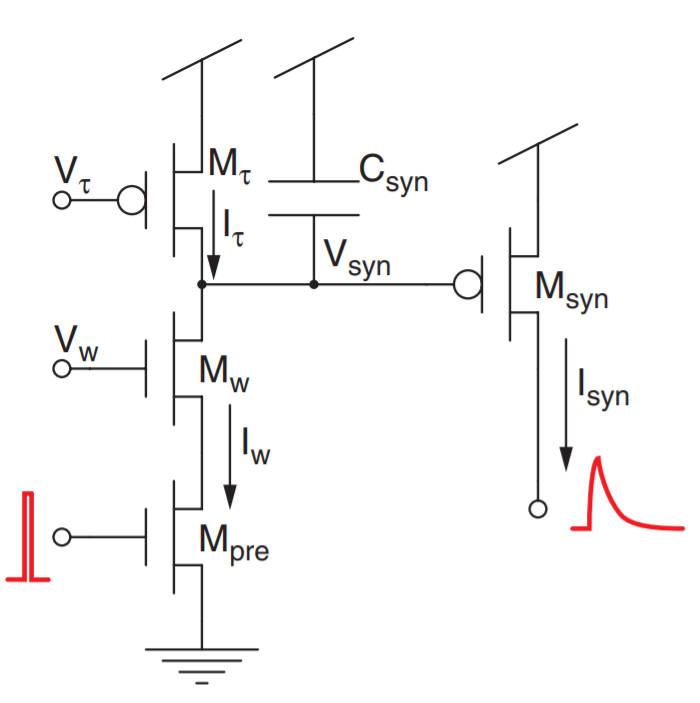
\includegraphics[width=.6\linewidth]{Figures/exponentially_decaying_integrator.PNG}
    \caption{Exponentially decaying integrator circuit.}
    \label{fig:exponentially_decaying_integrator}
\end{figure}

Figure \ref{fig:exponentially_decaying_integrator} shows the circuit of an exponentially decaying integrator that exploits the exponential behaviour of subthreshold MOSFETs and shows similar behaviour to a synapse. We assume that all transistors operate in subthreshold and in saturation. Consequently, we get the following equations for the circuit's currents:

\begin{equation}
    I_w = I_0 e^{\frac{\kappa V_w}{U_T}}
\end{equation}
\begin{equation}
    I_{\tau} = I_0 e^{\frac{\kappa (V_{dd}-V_{\tau})}{U_T}}
\end{equation}
\begin{equation}
    I_c = C \frac{d}{dt} (V_{dd}-V_{syn})
\end{equation}
\begin{equation}
    I_{syn} = I_0 e^{\frac{\kappa (V_{dd}-V_{syn})}{U_T}}
\end{equation}

Let's go through the circuit's behaviour step by step. We assume that initially the capacitor is fully charged, so $V_{syn} = V_{dd}$. As $V_{syn}$ is also the gate voltage of the pFET $M_{syn}$, this means that there is no current $I_{syn}$ flowing. When we get a pulse input, i.e. a positive gate voltage at transistor $M_{pre}$, we generate a current flow. The strength of the current is dependent on the gate voltage of the above transistor $M_w$ and we therefore denote the generated weighted current as $I_w$. You might wonder why we use two transistors to generate our weighted input. By separating our weight factor from the input pulse, we are able to process digital inputs that are either completely on or completely off. Additionally, we can introduce dynamic behaviour to our weighting factor $V_w$. This will be introduced in more detail in section \ref{sec:short_term_depression}. We can assume that our genereated input current $I_w$ is always significantly larger than the current $I_{\tau}$. Consequently, we have a constant current flowing out of the capacitor, i.e. discharging it, and a linear decrease of $V_{syn}$. This decrease leads to $V_{gs} > 0$ in the pFET $M_{syn}$ and we get an output current $I_{syn}$. When there is no pulse input at $M_{pre}$ anymore, no current $I_w$ is flowing. The current $I_{\tau}$ now flows into the capacitor and linearly charges $V_{syn}$ until it reaches $V_{dd}$ again. Due to the exponential relationship, the linear increase of $V_{syn}$ causes an exponential decrease of $I_{syn}$ until the output is completely shut off. The charge and discharge phase of the circuit can be described by the following equations:

\begin{equation}
    I_{syn}(t) = 
    \begin{cases}
      I_{syn}^- e^{+\frac{(t-t_i^-)}{\tau_c}& \text{(charge phase)}\\
      I_{syn}^+ e^{-\frac{(t-t_i^+)}{\tau_d}& \text{(discharge phase)}
    \end{cases}       
\end{equation}

We can rewrite the equation for $I_{syn}$ as follows:

\begin{equation}
    I_{syn}(t) = I_0 e^{n\Delta t (\frac{1}{\tau_c}+\frac{1}{\tau_d})-\frac{t}{\tau_d}} = I_0 e^{-\frac{\tau_c -f\Delta t (\tau_c + \tau_d)}{\tau_c \tau_d} t}
\end{equation}

where $n$ is the number of input spikes and $f = \frac{n}{t}$ the spike frequency. Note that for a large spike frequency, the capacitor does not have the time to charge up again. The voltage $V_{syn}$ eventually saturates at 0 and the resulting output current $I_{syn}$ becomes constant and independent of the input spikes. Looking at the above equation of $I_{syn}$, this is the case when the exponent becomes a positive value and eventually "explodes". We therefore get the following condition for our spike frequency:

\begin{equation}
    f \Delta t (\tau_c + \tau_d) > \tau_d \implies f < (\frac{\tau_c}{\tau_c+\tau_d}) \frac{1}{\Delta t}
\end{equation}

% Note that we separate input and weight in order to allow digital input while still being able to control the strength of I_w